\documentclass[../main.tex]{subfiles}
\begin{document}
\section{Introduction}
\label{sec:intro}
Building block level visualization libraries implement the functions that transform data into some component of the visual representation, providing a collection of components and utilities that can be combined to create a visualization \cite{wongsuphasawatNavigatingWideWorld2021}. Often domain specific tools are built out of these building block libraries, meaning the building block libraries must provide components general enough to satisfy a wide variety of data and visual representation needs. Specifically they must satisfy confirmatory and exploratory visualization needs \cite{tukeyWeNeedBoth1980}, in scientific and information (formal and informal\cite{pousmanCasualInformation2007}) visualization domains. To satisfy ever developing visualization needs, new components can be incorporated into the library in sometimes ad-hoc ways that can lead to API incoherancy and inconsistent behavior. We propose that like physical building blocks, building block libraries should provide a collection of well defined pieces that can be composed in whichever ways the blocks fit together.\note{figure of what we mean by building block?} We specify that for a valid visualization block is a structure preserving transformation from data to visual space, and we define structure in terms of \textit{continuity} and \textit{equivariance}. We then use this model to develop a design specification for the components of a building block visualization library. The notion of self contained, inherently modular, building blocks lends itself naturally to a functional paradigm of visualization \cite{hughesWhyFunctionalProgramming1989}. We adopt a functional model for a redesign because the lack of side effects means functional architecture can be evaluated for correctness, functional programs tend to be shorter and clearer, and are well suited to distributed, concurrent, and on demand tasks\cite{huHowFunctionalProgramming2015}.

This work is strongly motivated by the needs of the Matplotlib\cite{hunterMatplotlib2DGraphics2007,hunterArchitectureOpenSource} visualization library. One of the most widely used visualization libraries in Python, since 2002 new components and features have been added in a some what adhoc, sometimes hard to maintain, manner. Particularly, each new component carries its own implicit notion of how it believes the data is structured-for example if the data is a table, cube, image, or network - that is then expressed in the API for that component. In turn, this yields an inconsistent API for interfacing with the data, for example when  updating streaming visualizations or constructing dashboards\cite{a.sarikayaWhatWeTalk2019}. This entangling of data model with visual transform also yields inconsistencies in how visual component transforms, e.g. shape or color, are supported. We propose that these issues can be ameliorated via a redesign of the functions that convert data to graphics, named \textit{Artists} in Matplotlib, in a manner that reliably enforces \textit{continuity} and \textit{equivariance} constraints. We evaluate our functional model by implementing new artists in Matplotlib that are specified via \textit{equivariance} and \textit{continuity} constraints. We then use the common data model introduced by the model to demonstrate how plotting functions can be consolidated in a way that makes clear whether the difference is in expected data structure, visual component encoding, or the resulting graphic. 

\section{Background}
The notion that visualization is structure preserving maps from data to visual representation is neither a new formalism nor a new implementation goal; this work bridges the formalism and implementation in a functional manner with a topological approach at a building blocks library level to propose a new model that can be used to guide library development. 

\subsection{Structure: \textit{equivariance} \& \textit{continuity}}
\label{sec:intro_viz}
Visual representations of data, by definition, reflect something of the underlying structure and semantics\cite{friendlyBriefHistoryData2008}, whether through direct mappings from data into visual elements or via figurative representations that have meaning due to their similarity in shape to external concepts \cite{byrneAcquiredCodesMeaning2016}. The components of a visual representation were first codified by Bertin\cite{bertinSemiologyGraphicsDiagrams2011a}, who introduced a notion of structure preservation that we formally describe in terms of \textit{equivariance} and \textit{continuity}. 
 
\begin{figure}[H]
        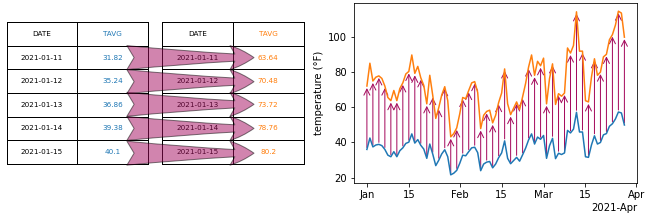
\includegraphics[width=1\columnwidth]{figures/intro/equivariance.png}
        \caption{The data in blue is scaled by a factor of two, yielding the data in orange. To preserve \textit{equivariance}, the blue line plot representation of the unscaled data is also scaled by a factor of two, yielding the orange line plot that is equivalent to the scaled data.}
        \label{fig:intro:equivariance}
\end{figure}
Bertin proposes that there are classes of visual encodings-such as position, shape, color, and texture-that when mapped to from specific types of measurement, quantitative or qualitative, will preserve the properties of that measurement type. For example, in \autoref{fig:intro:equivariance}, the data and visual representation are scaled by equivalent factors of two, resulting in the change illustrated in the shift from blue to orange data and lines. The idea of equivariance is formally defined as the mapping of a binary operator from the data domain to the visual domain in Mackinlay's \textit{A Presentation Tool}(APT) model\cite{mackinlayAutomatingDesignGraphical1986, mackinlayAutomaticDesignGraphical1987}. The algebraic model of visualization proposed by Kindlmann and Scheidegger uses equivariance to refer generally to invertible binary transformations\cite{kindlmannAlgebraicProcessVisualization2014}, which are mathematical groups \cite{shadrachIntroductionGroups2017}. Our model defines \textit{equivariance} in terms of monoid actions, which are a more restrictive set than all binary operations and more general than groups. As with the algebraic model, our model also defines structure preservation as commutative mappings from data space to representation space to graphic space, but our model uses topology to explicitely include continuity.

\begin{figure}[H]
    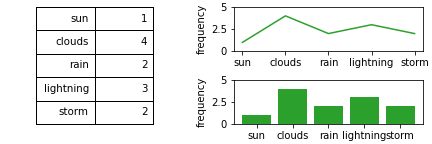
\includegraphics[width=1\textwidth]{figures/intro/continuity.png}
    \caption{The line plot does not preserve \textit{continuity} because it implies that the discrete records are connected to each other, while the bar plot is \textit{continuity} preserving because it visually represents the records as independent data points. }
    \label{fig:intro:continuity}
\end{figure}
Bertin proposes that the visual encodings be composited into graphical marks that match the \textit{continuity} of the data - for example discrete data is a point, 1D continuous is the line, and 2D data is the area mark. In \autoref{fig:intro:continuity}, the line plot does not preserve continuity because the line connecting the discrete categories implies that the frequency of weather events is sampled from a continuous interval and the categories are points on that interval. \note{transition statement}

\begin{mdframed}[roundcorner=10pt, frametitle=Structure, frametitlerule=true, frametitlebackgroundcolor=gray!10]
    \begin{description}
        \item[\textbf{continuity}] How records in the dataset are connected to each other, e.g. discrete rows, neworked nodes, points on a continuous surface
        \item[\textbf{equivariance}] if an action is applied to the data or the graphic--e.g. a rotation, permutation, translation, or rescaling-- there must be an equivalent action applied on the other side of the transformation. 
    \end{description}
\end{mdframed}

The measure of how much of the structure of the data the graphic encodes is a concept Mackinlay termed expressiveness, while the graphic's effectiveness describes how much design choices are made in deference to perceptual saliency \cite{clevelandResearchStatisticalGraphics1987,clevelandGraphicalPerceptionTheory1984,chambersGraphicalMethodsData1983a, munznerVisualizationAnalysisDesign2014}. When the properties of the representation match the properties of the data, then the visualization is easier to understand according to Norman's Naturalness Principal\cite{NaturalnessPrincipleInfoVis}. These ideas are combined into Tufte's notion of graphical integrity, which is that a visual representation of quantitative data must be directly proportional to the numerical quantities it represents (Lie Principal), must have the same number of visual dimensions as the data, and should be well labeled and contextualized, and not have any extraneous visual elements \cite{tufteVisualDisplayQuantitative2001}. 



\subsection{Tools}
\label{sec:intro_data_tools}

One of the reasons we developed a new formalism rather than adopting the architecture of an existing library is that most information visualization software design patterns, as categorized by Heer and Agrawala\cite{HeerSoftware2006}, are tuned to very specific data structures. This in turn restricts the design space of visual algorithms that display information (the visualization types the library supports) since the algorithms are designed such that the structure of data is assumed, as described in Tory and Möller's taxonomy \cite{ToryRethinkingVisualization2004}. In proposing a new architecture, we contrast the trade offs libraries make, describe different types of data continuity, and discuss metrics by which a visualization library is traditionally evaluated. 

\begin{figure}[H]
    \begin{subfigure}{.3\textwidth}
        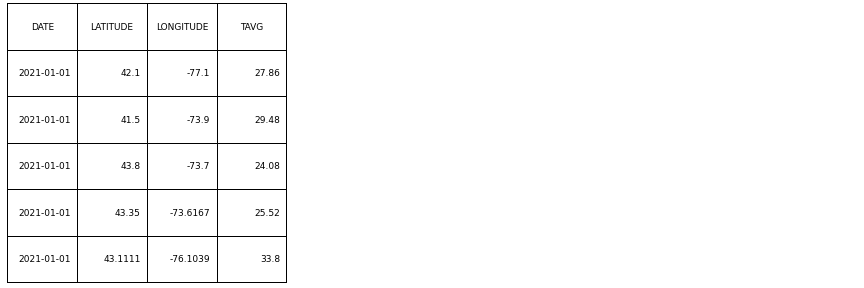
\includegraphics[width=2.75\textwidth]{figures/intro/table_only.png}
    \end{subfigure}
    \begin{subfigure}{.3\textwidth}
        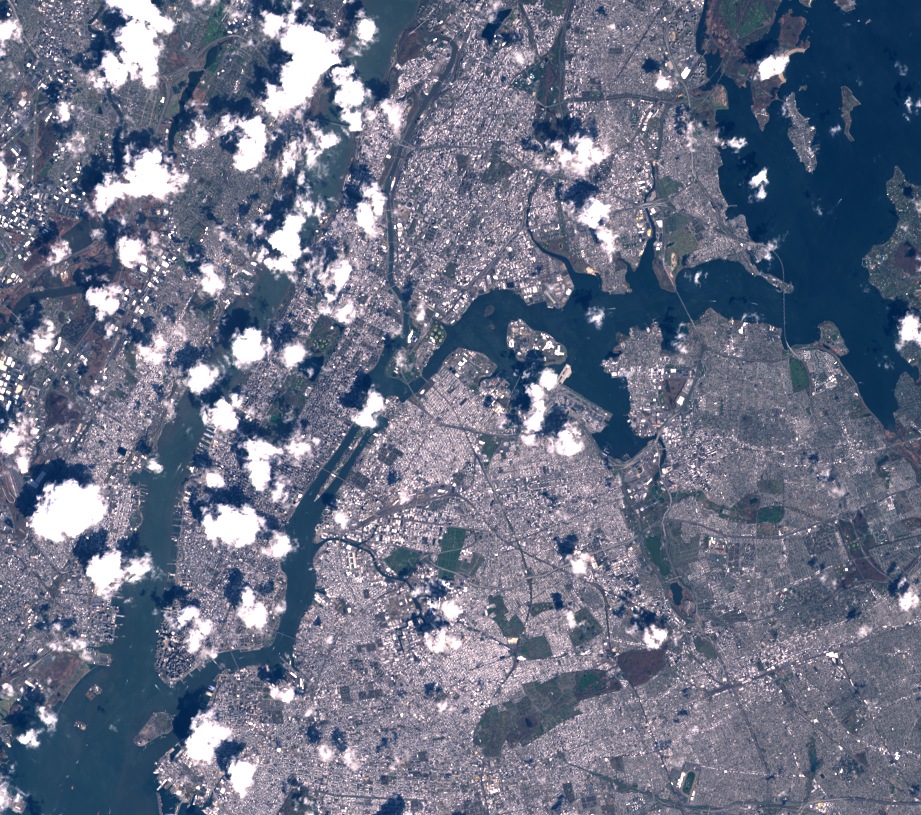
\includegraphics[width=1\textwidth]{figures/intro/landsat.png}
    \end{subfigure}
    \begin{subfigure}{.3\textwidth}
        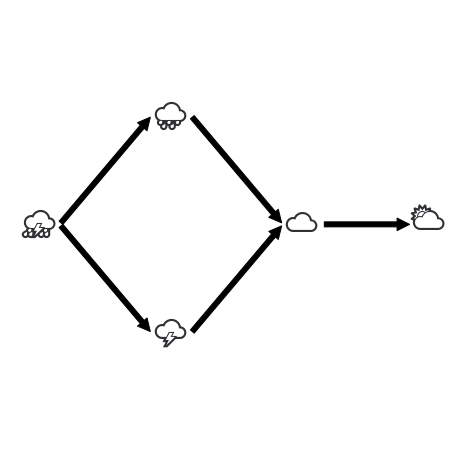
\includegraphics[width=1\textwidth]{figures/math/graph.png}
    \end{subfigure}
    \caption{Visualization libraries, especially ones tied to specific domains, tend to be architectured around a core data structure, such as tables, images, or networks. }
\end{figure}

One extensive family of relational table based libraries are those based on Wilkenson's Grammar of Graphics (GoG) \cite{wilkinsonGrammarGraphics2005}, including ggplot\cite{wickhamGgplot2ElegantGraphics2016a}, protovis\cite{bostockProtoviz2009} and D3 \cite{bostockDataDrivenDocuments2011}, vega\cite{satyanarayanDeclarativeInteractionDesign2014} and altair\cite{vanderplasAltairInteractiveStatistical2018}. The restriction to tables in turn restricts the native design space to visualizations suited to tables. Since the data space and graphic space is very well defined in this grammar, it lends itself to a declarative interface \cite{heerDeclarative2010}. This grammar oriented approach allows users to describe how to compose visual elements into a graphical design \cite{wongsuphasawatNavigatingWideWorld2021}, while we are proposing a framework for building those elements. An example of this distinction is that the GoG grammar includes computation and aggregation of the table as part of the grammar, while we propose that most computations are specific to domains and only try to describe them when they are specifically part of the visual encoding - for example mapping data to a color. Disentangling the computation from the visual transforms allows us to determine whether the visualization library needs to handle them or if they can be more efficiently computed by the data container.


A different class of user facing tools are those that support images, such as ImageJ\cite{schneiderNIHImageImageJ2012} or Napari\cite{nicholas_sofroniew_2021_4533308}. These tools often have some support for visualizing non image components of a complex data set, but mostly in service to the image being visualized. These tools are ill suited for general purpose libraries that need to support data other than images because the architecture is oriented towards building plugins into the existing system \cite{WritingPlugins} where the image is the core data structure. Even the digital humanities oriented ImageJ macro ImagePlot\cite{studiesCulturevisImageplot2021}, which supports some non-image aggregate reporting charts, is still built around image data as the primary input. 


\begin{figure}[H]
    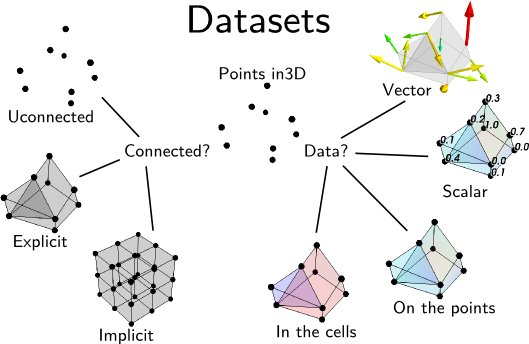
\includegraphics[width=1\textwidth]{figures/intro/dataset_diagram.png}
    \caption{One way to describe data is by the connectivity of the points in the dataset. A database for example is often discrete unconnected points, while an image is an implicitely connected 2D grid. This image is from the Data Representation chapter of the MayaVi 4.7.2 documentation.\cite{DataRepresentationMayavi}}
    \label{fig:intro_data_format}
\end{figure}

There are also visualization tools where there is no single core structure, and instead internally carry around many different representations of data. Matplotlib, has this structure, as does VTK \cite{hanwellVisualizationToolkitVTK2015,geveci2012vtk} and its derivatives such as MayaVi\cite{RamachandranMayaVI2011} and extensions such as ParaView\cite{ahrens2005paraview} and the infoviz themed Titan\cite{brianwylieUnifiedToolkitInformation2009}. Where GoG and ImageJ type libraries have very consistent APIs for their visualization tools because the data structure is the same, the APIs for visualizations in VTK and Matplotlib are significantly dependent on the structure of the data it expects. VTK has explicitely codified this in terms of continuity based data representations, as illustrated in figure~\ref{fig:intro_data_format}. This in turn means that every new type of visualization must carry implicit assumptions about data structure in how it interfaces with the input data. This has lead to poor API consistency and brittle code as every visualization type has a very different point of view on how the data is structured. This API choice particularly breaks down when the same dataset is fed into visualizations with different assumptions about structure or into a dashboard consisting of different types of visualization\cite{a.sarikayaWhatWeTalk2019,fewDashboardConfusionRevisited2007} because there is no consistent way to update the data and therefore no consistent way of guaranteeing that the views stay in sync. Our model is a structure dependent formalism, but then also provides a core representation of that structure that is abstract enough to provide a common interface for many different types of visualization.

\subsection{Data}
\label{sec:intro_data}
Discrete and continuous data and their attributes form a discipline independent design space \cite{pousmanCasualInformation2007}, so one of the drivers of this work was to facilitate building libraries that could natively support domain specific data containers that do not make assumptions about data continuity. As shown in figure~\ref{fig:intro_data_format}, there are many types of connectivity. A database typically consists of unconnected records, while an image is an implicit 2D grid and a network is some sort of explicitly connected graph. These data structures typically contain not only the measurements or values of the data, but also domain specific semantic information such as that the data is a map or an image that a modern visualization library could exploit if this information was exposed to the API. 

\begin{figure}[H]
    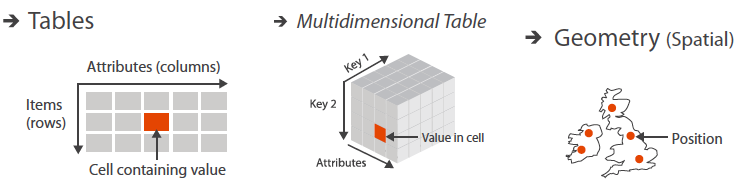
\includegraphics[width=1\textwidth]{figures/intro/munzner_datatypes.png}
    \caption{Image is figure 2.8 in Munzner's Visualization Analysis and Design\cite{munznerVisualizationAnalysisDesign2014}}
\end{figure}

As shown in figure~\ref{fig:intro_data_format}, there are many distinct ways of encoding each specific type of structure, while as mentioned in section~\ref{sec:intro_data_tools} APIs are clearer when structured around a common data representation. Fiber bundles were proposed by Butler as one such representation because they encode the continuity of the data separately from the types of variables and are flexible enough to support discrete and ND continuous datasets \cite{butlerVisualizationModelBased1989,butlerVectorBundleClassesForm1992}. Since Butler's model lacks a robust way of describing variables, we fold in Spivak's Simplicial formulation of databases \cite{spivakDatabasesAreCategories2010,spivakSIMPLICIALDATABASES} so that we can encode a schema like description of the data in the fiber bundle. In this work we will refer to the points of the dataset as \textit{records} to indicate that a point can be a vector of heterogenous elements. Each \textit{component} of the record is a single object, such as a temperature measurement, a color value, or an image. We also generalize \textit{component} to mean all objects in the dataset of a given type, such as all temperatures or colors or images. The way in which these records are connected is the \textit{connectivity}, \textit{continuity}, or more generally \textit{topology}.

\begin{mdframed}[roundcorner=10pt, frametitle= definitions, frametitlerule=true, frametitlebackgroundcolor=gray!10]
    \begin{description}
        \item[\textbf{records}] points, observations, entries 
        \item[\textbf{components}] variables, attributes, fields 
        \item[\textbf{connectivity}] how the records are connected to each other
    \end{description}
\end{mdframed}

Often this topology has metadata associated with it, describing for example dependent variables and the independent variables they are dependent on, or information about the structure of the data such as when and where the measurement was taken. Building on the idea of metadata as \textit{keys} and their associated \textit{values} proposed by Munzner \cite{munznerChDataAbstraction}, we propose that information rich metadata are part of the components and instead the values are keyed on coordinate free structural ids. In contrast to Munzner's model where the semantic meaning of the key is tightly coupled to the position of the value in the dataset, our model considers keys to be a pure reference to topology. This allows the metadata to be altered, for example by changing the coordinate systems or time resolution, without imposing new semantics on the underlying structure.



\subsection{Contribution}
This work presents a mathematical model of the transformation from data to graphic representation and a proof of concept implementation. Specifically, the contributions of this work are 
\begin{enumerate}
    \item a formal description of the topology preserving relationship between data and graphic via continuous maps
    \item a formal description of the property preservation from data component to visual representation as equivariant maps that carry a homomorphism of monoid actions
    \item abstraction of data structure using fiber bundles with schema like fibers to encode components and topology 
    \item algebraic sum operator such that more complex visualizations can be built from simple ones 
    \item a functional oriented visualization tool architecture built on the mathematical model to demonstrate the utility of the model
    \item a prototype of the architecture built on Matplotlib's infrastructure to demonstrate the feasibility of the model
\end{enumerate}
In contrast to mathematical models of visualization that aim to evaluate visualization design, we propose a topological framework for building tools to build visualizations. We defer judgement of expressivity and effectiveness to developers building domain specific tools, but provide them the framework to do so. 
\end{document}